\documentclass[12pt]{article}
\usepackage[utf8]{inputenc}
\usepackage{fullpage}
\usepackage{color}
\usepackage{listings}
\usepackage{graphicx}
\title{CSC 431 Compiler Report}
\date{}
\author{Austin Wise, Ryan Schroeder}

\begin{document}
\maketitle
\tableofcontents

\pagebreak

\section{Architecture}

A small data flow engine hooks all the pieces of the compiler together.
First we parse the command line arguments.
Based on the values we obtain from the argument parser we construct a tree of tasks that represents the actions we are going to perform.
The nodes in the tree represent the actions, the edges pass data from one node to its dependants.
Next, using our Step.DoAll function we execute each step in a topological sorted order.

\begin{figure}
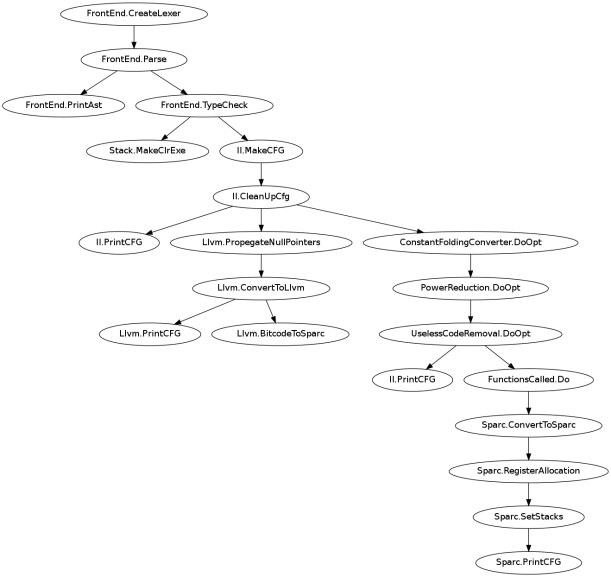
\includegraphics{compSteps.png}
\caption{Handling the two exceptions.}
\label{success}
\end{figure}

	
\pagebreak

\section{Representation of Key Data}


\subsection{Instructions}
base instruction class has source and destination sources to assist with optimizations and register allocation
for each instruction type we use a T4 template to generate specific subclasses for each individual instruction
these templates also generate a miloc converter and imiloc translator to aid in translating miloc to sparc

\subsection{Control Flow Graph}
base node class represents abstract node
specific nodes for if/loop/basic blocks/series of nodes
all nodes have a generic type parameter to ensure that they only hold instructions of one type, e.g. sparc/miloc
all nodes in the control flow graph have the ability to copy their structure while at the same time applying a supplied implementation of the IInstructionConverter Interface to convert instructions in basic blocks from one type of instruction to another
this facility is used both for converting between instruction types and for doing code transformations on a single instruction type.
the IInstructionConverter allows n:m mapping between instructions. the code is sexy, look at it.

\section{Optimizations Implemented}

\subsection{Constant Folding}
First we traverse each basic block and we determine if we can find a constant value for the result of an instruction.
As we traverse the basic blocks we store two tables of values, one global table representing instructions that have constant values, and a local table.
The local table is constantly being updated with values of registers that are known at the current point in the instruction stream.
When we encounter an unknown instruction we remove all of its destination registers from the local table.
After traversing each block individually we iteratively visit each block again looking for cross block constant expressions until we can find no more.
We use reaching definitions of the source registers to check if they have a constant value.
The resulting map of instructions to constant values is used by ConstantFoldingConverter (an implementation of IInstructionConverter) to replace the instructions with loads.
\subsection{Power Reduction}
power reduction and shit
\subsection{Useless Code Removal}
useless code removal and shit
\section{Performance of the Benchmarks}
  
\end{document}
